%%%%%%%%%%%%
%
% $Autor: Adhiraj, Sudheshna,Srikhant $
% $Datum: 2024-12-25 08:03:15Z $
% $Pfad: TemplateSensor $
% $Version: 4250 $
% !TeX spellcheck = en_GB/de_DE
% !TeX encoding = utf8
% !TeX root = filename 
% !TeX TXS-program:bibliography = txs:///biber
%
%%%%%%%%%%%%

% Structure
\chapter{Sensor/Actor}

\section{Accelerometer}

\subsection{Description}
The accelerometer enables significant motion detection (SMD), which recognizes large-scale movements. SMD can be used to activate specific device functions, such as waking the system from sleep mode or triggering predefined actions based on significant gestures.\cite{Zhou:2020}

The LSM9DS1 is a versatile and energy-efficient IMU with advanced sensing capabilities, supporting a range of applications where motion detection, orientation tracking, and gesture recognition are essential. Its compact design, low power consumption, and robust environmental tolerance make it a reliable choice for portable, battery-powered devices like the Magic Wand.\cite{Zhou:2020}
	
An \ac{imu} consists of three sensors that measure an object's orientation, position, vibration and movement in 3D space in real-time. These sensors are typically arranged in a pattern, including a tri-axial accelerometer, gyroscope, and magnetometer\cite{Ahmad:2013}. An accelerometer is used to measure the change in velocity of a moving or vibrating object\cite{Ahmad:2013}. Gyroscope measures the angular rotation\cite{Ahmad:2013}. A Magnetometer is used to measure yaw angle rotation, calibrating to the gyroscope data to improve the big drift issue\cite{Ahmad:2013}. 

The accelerometer functions by gauging the acceleration (Ax, Ay, Az), which denotes the rate of acceleration change over time. The acceleration values along each axis are conventionally expressed in units of meters per second squared $(m/s^2)$ \cite{Vernier:2023}. To illustrate, if the LSM9DS1 records an acceleration of 15 $m/s^2$ along the x-axis, this signifies that the object under observation is experiencing a velocity increment of 15 meters per second every second in the x-direction.
\subsection{Specific Sensors}
\textbf{Tilt Detection}
Using the accelerometer, the IMU can detect orientation changes with minimal power usage. Tilt detection is particularly useful for identifying subtle shifts in position, enhancing the responsiveness of gesture-based controls.\cite{Zhou:2020}

\textbf{Significant Motion Detection}
The accelerometer enables significant motion detection (SMD), which recognizes large-scale movements. SMD can be used to activate specific device functions, such as waking the system from sleep mode or triggering predefined actions based on significant gestures.\cite{Zhou:2020}

The LSM9DS1 is a versatile and energy-efficient IMU with advanced sensing capabilities, supporting a range of applications where motion detection, orientation tracking, and gesture recognition are essential. Its compact design, low power consumption, and robust environmental tolerance make it a reliable choice for portable, battery-powered devices like the Magic Wand.\cite{Zhou:2020}
	
An \ac{imu} consists of three sensors that measure an object's orientation, position, vibration and movement in 3D space in real-time. These sensors are typically arranged in a pattern, including a tri-axial accelerometer, gyroscope, and magnetometer\cite{Ahmad:2013}. An accelerometer is used to measure the change in velocity of a moving or vibrating object\cite{Ahmad:2013}. Gyroscope measures the angular rotation\cite{Ahmad:2013}. A Magnetometer is used to measure yaw angle rotation, calibrating to the gyroscope data to improve the big drift issue\cite{Ahmad:2013}. 

The accelerometer functions by gauging the acceleration (Ax, Ay, Az), which denotes the rate of acceleration change over time. The acceleration values along each axis are conventionally expressed in units of meters per second squared $(m/s^2)$ \cite{Vernier:2023}. To illustrate, if the LSM9DS1 records an acceleration of 15 $m/s^2$ along the x-axis, this signifies that the object under observation is experiencing a velocity increment of 15 meters per second every second in the x-direction.

\subsection{Specification}
\subsection{Library}
Details about libraries used to interface with accelerometers (e.g., Adafruit Sensor Library, Arduino libraries).
Installation process and setup.
Features provided by these libraries (e.g., data acquisition, filtering, scaling).
\begin{verbatim}
// Include the necessary libraries
#include <Wire.h>
#include <Adafruit_Sensor.h>
#include <Adafruit_LSM9DS1.h>
\end{verbatim}
\subsection{Functions}
\begin{verbatim}
// Check if acceleration data is available
if (IMU.accelerationAvailable()) {
	// Read the acceleration values
	IMU.readAcceleration(x, y, z);
	
	// Print the acceleration values
	Serial.print("AccX: ");
	Serial.print(x);
	Serial.print(", AccY: ");
	Serial.print(y);
	Serial.print(", AccZ: ");
	Serial.println(z);
}

\end{verbatim}
\subsection{Calibration}
Steps for calibrating an accelerometer:
\begin{itemize}
	\item Importance of calibration for accelerometer sensors.
	\item Methods for calibrating accelerometers (e.g., zeroing, scaling, temperature compensation).
	\item Tools and techniques for accelerometer calibration (e.g., software tools, calibration kits).
\end{itemize}

\subsection{Simple Code}
\begin{verbatim}
		#include <Wire.h>
		#include <Adafruit_Sensor.h>
		#include <Adafruit_LSM9DS1.h>

		// Create LSM9DS1 object
		Adafruit_LSM9DS1 lsm = Adafruit_LSM9DS1();

		void setup() {
		// Start the Serial Monitor
		Serial.begin(115200);

		// Initialize the LSM9DS1
		if (!lsm.begin()) {
			Serial.println("Failed to initialize LSM9DS1! Check wiring.");
			while (1);
		}

		// Set accelerometer range (default is ±2g)
		lsm.setupAccel(lsm.LSM9DS1_ACCELRANGE_2G);  
		// Options: 2G, 4G, 8G, 16G

		// Optional: Set accelerometer data rate (default is 119 Hz)
		lsm.setupAccelDataRate(lsm.LSM9DS1_ACCELDATARATE_119HZ);
		}

		void loop() {
		// Read accelerometer data
		sensors_event_t accelEvent;
		lsm.getEvent(&accelEvent, NULL, NULL);  
		// Get accelerometer event data only

		// Print accelerometer readings (in m/s²)
		Serial.print("Accel X: ");
		Serial.print(accelEvent.acceleration.x);
		Serial.print(" m/s², Y: ");
		Serial.print(accelEvent.acceleration.y);
		Serial.print(" m/s², Z: ");
		Serial.print(accelEvent.acceleration.z);
		Serial.println(" m/s²");

		// Delay to make output more readable
		delay(100);
		}

\end{verbatim}
\subsection{Applications}
Practical uses of accelerometers:
\begin{itemize}
	\item In smartphones (e.g., screen orientation, motion detection).
	\item Automotive industry (e.g., airbag deployment, stability control).
	\item Robotics (e.g., navigation, balance).
	\item Wearable devices and fitness trackers.
	\item Industrial applications (e.g., vibration monitoring, machine diagnostics).
\end{itemize}
\subsection{Tests}
Techniques to test an accelerometer’s functionality:
This is the C++ code for testing the accelerometer on the Arduino Nano 33 BLE Sense using the \texttt{Adafruit\_LSM9DS1} library. 

\begin{figure}[h!]
	\centering
	\begin{lstlisting}[style=pythonstyle ,language=C++, caption={Testing the accelerometer}, label={lst:arduino_accelerometer}]
		#include <Wire.h>
		#include <Adafruit_Sensor.h>
		#include <Adafruit_LSM9DS1.h>
		
		// Create an instance of the LSM9DS1 sensor
		Adafruit_LSM9DS1 lsm = Adafruit_LSM9DS1();
		
		void setup() {
			// Start serial communication
			Serial.begin(115200);
			
			// Initialize the LSM9DS1 sensor
			if (!lsm.begin()) {
				Serial.println("Could not find a valid LSM9DS1 sensor, check wiring!");
				while (1);
			}
			
			Serial.println("LSM9DS1 test initialized.");
		}
		
		void loop() {
			// Read accelerometer data
			sensors_event_t event;
			lsm.getEvent(&event);
			
			// Print accelerometer values
			Serial.print("X: ");
			Serial.print(event.acceleration.x);
			Serial.print(" Y: ");
			Serial.print(event.acceleration.y);
			Serial.print(" Z: ");
			Serial.println(event.acceleration.z);
			
			// Delay before the next reading
			delay(1000);
		}
	\end{lstlisting}
	\caption{C++ code for testing the accelerometer on the Arduino Nano 33 BLE Sense.}
	\label{lst:cpp_code}
\end{figure}

This is the Python code for reading the accelerometer data from the Arduino via serial communication. The \texttt{pyserial} library is required for this script.

\begin{figure}[h!]
	\centering
	\begin{lstlisting}[style=pythonstyle ,language=python, caption={Accelerometer testing in pyserial}, label={lst:arduino_accelerometer}]
		import serial
		import time
		
		# Replace with the correct port for your system (e.g., 'COM3' on Windows or '/dev/ttyACM0' on Linux)
		arduino_port = '/dev/ttyACM0'  
		baud_rate = 115200
		
		# Establish connection to the Arduino
		arduino = serial.Serial(arduino_port, baud_rate, timeout=1)
		time.sleep(2)  # Wait for Arduino to initialize
		
		# Function to read accelerometer data from the Arduino
		def read_accelerometer():
		while True:
		line = arduino.readline().decode('utf-8').strip()
		if line:
		print(line)
		
		# Start reading accelerometer data
		read_accelerometer()
	\end{lstlisting}
	\caption{Python code for reading accelerometer data from the Arduino Nano 33 BLE Sense.}
	\label{lst:python_code}
\end{figure}

\subsection{Further Readings}

\section{Gyroscope}
\subsection{Description}
The STMicroelectronics LSM9DS1 gyroscope is a precision instrument for measuring angular velocity around the x, y, and z axes. With adaptable measurement ranges of ±245, ±500, and ±2000 degrees per second (dps), the gyroscope is highly versatile for various applications such as inertial navigation, robotics, and drone stabilization.\cite{St:2024}
Key Features:
\begin{itemize}
\item Sampling Rates: The gyroscope offers adjustable sampling rates, allowing it to operate at frequencies of 14.9 Hz, 59.5 Hz, 119 Hz, 238 Hz, 476 Hz, or 952 Hz.\cite{St:2024} This flexibility ensures compatibility with a broad range of motion measurement requirements.

\item Voltage and Power Consumption: The gyroscope operates within a voltage range of 1.71 V to 3.6 V, making it suitable for different system configurations.\cite{St:2024} Its low power consumption—between 1 mA to 2 mA—enhances its suitability for portable, battery-operated devices.\cite{St:2024}

\item Compact Design: The LSM9DS1 integrates seamlessly into compact systems, offering engineers and designers a robust yet space-efficient solution.\cite{Maker:2024}

\item Operation Principle: The gyroscope operates based on Coriolis acceleration, a phenomenon observed when a vibrating object moves in a rotating reference frame. Piezoelectric crystals are used to detect changes in angular velocity by converting inertial forces into electrical signals.

\item Applications: The LSM9DS1 gyroscope is designed for:
\end{itemize}
Inertial Measurement Units (IMUs): Combined with accelerometers and magnetometers, it forms a 9-DOF motion tracking system.\cite{Ahmad:2013}
Drone Stabilization: Essential for real-time attitude adjustments.\cite{Ahmad:2013}
Navigation Systems: Key in applications like gyrocompasses or attitude heading reference systems.\cite{Ahmad:2013}

$$ \text{Angular velocity} = \left(\frac{\text{Gyroscope axis raw data}}{65536} \times \text{full scale Gyroscope range}\right) \frac{\circ}{\text{s}} $$

For example, if the gyroscope's raw data along the X axis is 16384 and the range is ±250°/s, the calculation for angular velocity along the X axis would be:

$$ \text{Angular velocity along the X axis} = \left(\frac{16384}{65536} \times 500\right) \frac{\circ}{\text{s}} = 125 \frac{\circ}{\text{s}} $$


\begin{figure}[H]\centering
	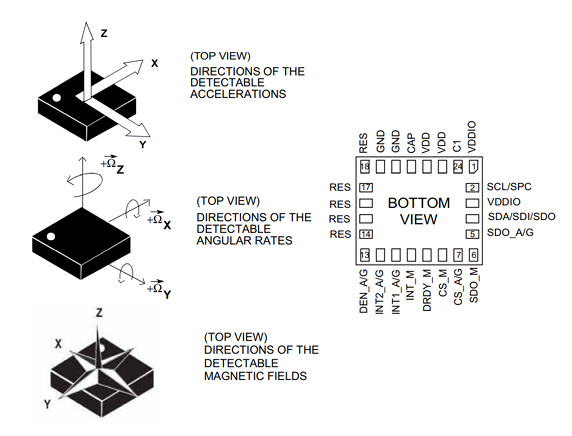
\includegraphics[width=0.8\textwidth]{Images/Sensor Actor/Gyroscope} 
	\caption{\textbf{Gyroscope}}
	\label{fig:Pin_assignment_of_Arduino_Nano_33_BLE_Sense} 
\end{figure}
\begin{figure}[H]\centering
	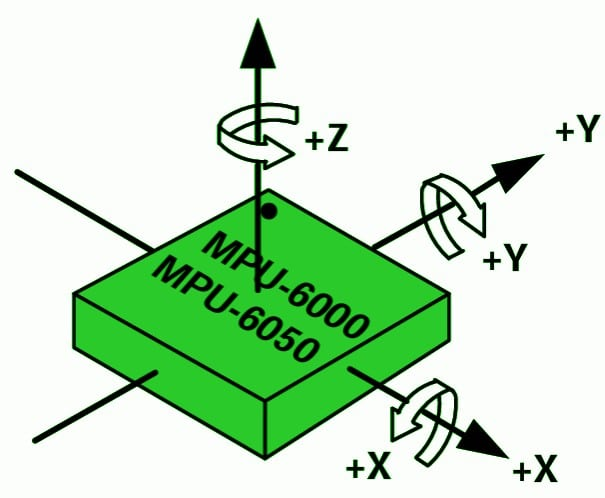
\includegraphics[width=0.8\textwidth]{Images/Sensor Actor/orientation_axes} 
	\caption{\textbf{Orientation Axes of Gyroscope}}
	\label{fig:Pin_assignment_of_Arduino_Nano_33_BLE_Sense} 
\end{figure}
\subsection{Specification}

	\textbf{Gyroscope Specifications of MPU6050:}\newline
	\begin{tabular}{|l|l|l|}
		\hline
		Full scale range & FS\_SEL & Range \\ \hline
		& 0 & ±250°/s \\ \hline
		& 1 & ±500°/s \\ \hline
		& 2 & ±1000°/s \\ \hline
		& 3 & ±2000°/s \\ \hline
		Sensitivity Scale Factor Tolerance & & ±3\% \\ \hline
		Gyroscope start-up time && 30 ms \\ \hline
		Output data rate & & 4 to 8000 Hz \\ \hline
	\end{tabular}

\subsection{Library}

{Description}
To meet the project's needs, three essential libraries must be integrated, each serving a specific purpose that ensures smooth operation and functionality of the system. Here's a breakdown of each library’s role:

\textbf{1. Wire.h:}
   This is an Arduino standard library used for I2C communication, a protocol that allows devices to communicate with each other using only two wires, reducing the complexity of wiring in systems that need to connect multiple devices. I2C is widely used for connecting sensors, displays, and other peripherals to a microcontroller. The `Wire.h` library simplifies interactions with I2C devices by handling the low-level details of communication. Developers can initialize the I2C bus, send and receive data, and manage multiple I2C devices on the same bus seamlessly. This is crucial for systems that need to manage several sensors or external modules, as it facilitates smooth and efficient data transfer.\cite{Passaro:2017}

\textbf{2. Kalman.h:}
   The Kalman filter is an advanced mathematical algorithm used to process noisy sensor data and provide more accurate estimates of a system’s state. The `Kalman.h` library allows developers to easily implement this filter into Arduino-based projects. It is particularly useful in applications where precise data is essential, such as robotics, control systems, and navigation. By filtering out noise and accounting for uncertainties in sensor readings, the Kalman filter improves the accuracy of measurements like position, velocity, and orientation, which are crucial in motion tracking, sensor fusion, or stabilizing systems like drones and robots.\cite{Passaro:2017}

\textbf{3. Arduino\_LSM9DS1.h:}
   This library is specifically designed to interface with the LSM9DS1 IMU (Inertial Measurement Unit) sensor, developed by STMicroelectronics. The LSM9DS1 combines three essential motion sensors in one package: an accelerometer, a gyroscope, and a magnetometer. The `Arduino\_LSM9DS1.h` library allows developers to easily access data from these sensors, such as acceleration, angular velocity, and magnetic field strength. Additionally, the library offers functions to configure sensor parameters like measurement ranges, sampling rates, and operating modes, enabling customization based on the needs of the application. This is particularly useful in systems that rely on accurate motion tracking or orientation sensing.\cite{Passaro:2017}

Together, these libraries enable the integration of multiple sensors into a cohesive system, facilitating communication, data processing, and precise motion measurement.

\subsection{Installation}
\begin{figure}[H]\centering
	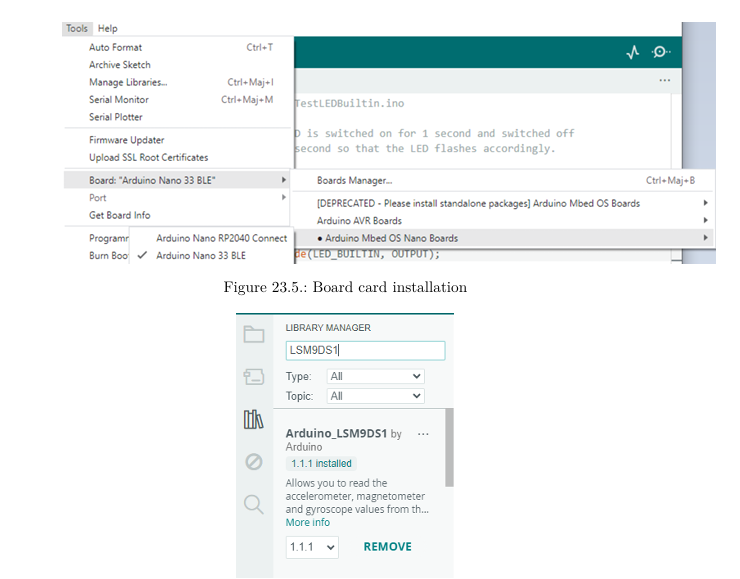
\includegraphics[width=0.8\textwidth]{Images/Sensor Actor/Installation} 
	\caption{\textbf{Installation of Libraries}}
	\label{fig:Pin_assignment_of_Arduino_Nano_33_BLE_Sense} 
\end{figure}
\begin{figure}[H]\centering
	
\includegraphics[width=0.8\textwidth]{Images/Sensor Actor/Installation_of_wire} 
	\caption{\textbf{Installation of wire.h}}
	\label{fig:Pin_assignment_of_Arduino_Nano_33_BLE_Sense} 
\end{figure}
\subsection{Functions}
The LSM9DS1 library for the Arduino Nano 33 BLE Sense provides a set of functions to interact with the LSM9DS1 IMU (Inertial Measurement Unit) sensor. The functions available depend on the communication protocol being used, either I2C or SPI.\cite{Passaro:2017}



\textbf{Function IMU.readGyroscope()}
The function IMU.readGyroscope() is used to retrieve data from an Inertial Measurement Unit's (IMU) gyroscope. It returns the angular velocity in degrees per second (dps), providing information about the rotational movement detected by the IMU. This data is crucial for applications like robotics, motion tracking, and navigation systems, where precise orientation control and stabilization are required.
The function typically returns x, y, and z values, representing the angular velocity along each of the three axes (x, y, and z). These values are floating-point numbers that describe the rotational velocity along each axis, enabling detailed tracking of changes in orientation. By regularly calling this function and analyzing the data over time, it becomes possible to monitor and respond to rotational movements accurately.
For example, in robotics, these readings can be used to adjust a robot’s position or orientation in real-time, while in drones, they assist with stabilization during flight.
\begin{code}[h!]
	\begin{Arduino}
  // Declare variables to store gyroscope data
  float x, y, z;
  
  // Check if gyroscope data is available
  if (IMU.gyroscopeAvailable()) {  
  	// Read the gyroscope data into variables x, y, z
  	IMU.readGyroscope(x, y, z);   
  	
  	// Print the x-axis angular velocity
  	Serial.print(x);               
  	
  	// Print a tab space for separation
  	Serial.print('\t');            
  	
  	// Print the y-axis angular velocity
  	Serial.print(y);               
  	
  	// Print another tab space for separation
  	Serial.print('\t');            
  	
  	// Print the z-axis angular velocity and move to the next line
  	Serial.println(z);             
  }
  
\end{Arduino}
\caption{Sample Code of IMU.readGyroscope()}\label{code:IMU.readGyroscope()}
\end{code}\newline
\textbf{Function IMU.gyroscopeAvailable()}
The function IMU.gyroscopeAvailable() is used to check whether new gyroscope data is available from the IMU. It returns a value of 1 if new data is ready to be retrieved, and 0 if no new data is available. This function is particularly useful in real-time applications, such as drone stabilization, virtual reality systems, or inertial navigation, where the system must determine whether to wait for updated gyroscope data or proceed with processing the available information.

For example, in a drone application, when the function returns 1, the system knows that new gyroscope data is available, and it can proceed to retrieve and use this information to adjust the drone's orientation or stabilize its motion. Conversely, a return value of 0 means that no new data has been received, prompting the system to wait until new data is available before continuing the process.

In the provided code example:\newline
\begin{code}[h!]
	\begin{Arduino}
	// Declare variables to store gyroscope data
	float x, y, z;
	
	// Check if gyroscope data is available
	if (IMU.gyroscopeAvailable()) {
		// Read the gyroscope data into variables x, y, z
		IMU.readGyroscope(x, y, z);
		
		// Print the x-axis angular velocity
		Serial.print(x);
		
		// Print a tab space for separation
		Serial.print('\t');
		
		// Print the y-axis angular velocity
		Serial.print(y);
		
		// Print another tab space for separation
		Serial.print('\t');
		
		// Print the z-axis angular velocity and move to the next line
		Serial.println(z);
	}
	
	\end{Arduino}
\caption{Sample Code of IMU.gyroscopeAvailable()}\label{code:IMU.gyroscopeAvailable()}
\end{code}
The program checks if new gyroscope data is available. If it is, the data is read and output to the serial monitor, showing the angular velocity along the x, y, and z axes.
This function is integral for applications that require continuous monitoring of rotational movement, ensuring that the system can react promptly to changes in orientation.

\textbf{Function IMU.gyroscopeSampleRate()}
The function IMU.gyroscopeSampleRate() is used to retrieve the rate at which the gyroscope integrated into the Inertial Measurement Unit (IMU) collects samples, typically expressed in Hertz (Hz). This sample rate indicates how frequently the gyroscope measures angular velocity, providing insights into its operational efficiency and performance.

\textbf{Sample Rate:} It is the frequency at which the gyroscope takes measurements. For example, a sample rate of 100 Hz means the gyroscope takes 100 readings per second.
\newline
\begin{code}[h!]
	\begin{Arduino}
	// Print the gyroscope sample rate
	Serial.print("Gyroscope sample rate= ");
	Serial.print(IMU.gyroscopeSampleRate());  // Print the gyroscope sample rate
	Serial.println("Hz");
	Serial.println();  // Print a blank line for separation
	
	// Print a label for angular speed in degrees/second
	Serial.println("Angular speed in degrees/second");
	
	// Print the axis labels with tab separation
	Serial.println("X\tY\tZ");
	
	\end{Arduino}
\caption{Sample Code of IMU.gyroscopeSampleRate()}\label{code:IMU.gyroscopeSampleRate()}
\end{code}	
\textbf{Function Breakdown:}
IMU.gyroscopeSampleRate(): This function returns the sample rate of the gyroscope in Hertz (Hz).
The Serial.print() functions then display the sample rate and additional information about the angular speed readings in degrees per second for the X, Y, and Z axes.

This function is especially useful in applications that require accurate and efficient motion tracking, such as drone stabilization, robotics, or virtual reality systems. Knowing the sample rate helps determine how often new data is available, which influences the system's ability to respond to changes in rotational movement.


\subsection{Calibration}
There are various methods to calibrate the sensors involved. It is necessary to know whether the sensor is balanced since the time between each calibration needs to be explicitly defined. Regular calibration should be done, especially when strange outputs are noticed. 

	Some methods of calibration are briefed below:
\begin{itemize}
\item
\textbf{Low and high limit method}\newline The low and high limit method involves recording minimum and maximum values on all three axes using a simple scratch to determine their absolute values. The sensor undergoes circular rotations along each axis multiple times. The centre point is then identified between these extremes.\cite{Gyroplace:2023}
Increasing the number of rotations enhances the likelihood of capturing the absolute peak. The center point will be close to zero if the sensor exhibits no offset. However, slight variations may indicate a hard iron offset attributed to distortion caused by the Earth’s magnetic field.\cite{Gyroplace:2023}
This method assumes minimal soft iron distortion, evident from the rounded outlines in the graph.\cite{Gyroplace:2023}
It is important to note that this method necessitates capturing values each time to prevent performance degradation due to component drift and aging sensors. For devices relying on primary batteries, calibration becomes essential after each battery change, as the battery inevitably serves as the main source of magnetic disturbance, and new batteries may behave differently from their predecessors.\cite{Gyroplace:2023}

\item
\textbf{Scale Factor and Non-Orthogonal Calibration}\newline With given initial attitude derived from alignment procedure, the gyroscope measurement can be integrated to calculate the orientation information through Strapdown inertial navigation algorithm. However, the computed attitude will drift over time and the error is gradually accumulated because of the sensor error. In stationary or low dynamic condition, the accelerometer output can be used to estimate the orientation relative to horizontal plane (i.e., pitch and roll).\cite{Gyroplace:2023} The attitude derived from accelerometer output is independent in different time epochs and not affected by accumulated error. Hence, based on the different sensors’ complimentary error propagation characteristics, we can make use of the accelerometer-derived attitude as reference signal to evaluate the attitude error introduced during integration process, and consequently determine the gyroscope error.\cite{Gyroplace:2023}
\end{itemize}
During the calibration process, the IMU is handheld by user and rotated along its axes slowly to avoid introducing external acceleration. The IMU orientation keeps varying during this procedure and the attitudes derived from different inertial sensors are compared to amend the attitude error and determine the sensor errors. A Kalman filter is designed to estimate the scale factor and non-orthogonal errors of gyroscope. The attitude error propagation equation, which includes sensor error, is utilized as the system dynamic model. The relationship between the accelerometer output and attitude error is modeled as the measurement equation.\cite{Gyroplace:2023}
\newline
\subsection{Simple Code}

Example IMU: Accelerometer and Gyroscope
\begin{code}
	\begin{Arduino}
		#include <Arduino_LSM9DS1.h>

		void setup() {
		Serial.begin(9600);

		// Initialize the IMU
		if (!IMU.begin()) {
			Serial.println("Failed to initialize IMU!");
			while (1); // Stop execution if initialization fails
		}
		}
		void loop() {
		float x, y, z;

		// Check if new acceleration data is available
		if (IMU.accelerationAvailable()) {
			IMU.readAcceleration(x, y, z);
			Serial.print("AccX: ");
			Serial.print(x);
			Serial.print(", AccY: ");
			Serial.print(y);
			Serial.print(", AccZ: ");
			Serial.println(z);
		}
		// Check if new gyroscope data is available
		if (IMU.gyroscopeAvailable()) {
			IMU.readGyroscope(x, y, z);
			Serial.print("GyroX: ");
			Serial.print(x);
			Serial.print(", GyroY: ");
			Serial.print(y);
			Serial.print(", GyroZ: ");
			Serial.println(z);
		}
		delay(1000); // Wait for 1 second before reading again
		}
	\end{Arduino}
	\caption{Example code for reading accelerometer and gyroscope data from the LSM9DS1 IMU}\label{code:IMU-example}
\end{code}

\subsection{Simple Application}
Gyroscopes in IMUs are essential for detecting and maintaining orientation and rotational motion in a wide range of devices:

\begin{itemize}
	\item \textbf{Smartphones/Tablets}: They enable features like screen auto-rotation and motion controls for gaming and virtual reality (VR).\cite{Passaro:2017}
	\item \textbf{Drones}: Gyroscopes stabilize flight by measuring angular velocity, allowing the drone to correct tilt and maintain stable orientation.\cite{Passaro:2017}
	\item \textbf{Robotics}: In robots, gyroscopes assist in balancing and navigation by tracking rotational movements, ensuring accurate motion control.\cite{Passaro:2017}
	\item \textbf{VR/AR}: In virtual and augmented reality systems, gyroscopes track head movement to provide an immersive experience by adjusting visuals based on real-time orientation.\cite{Passaro:2017}
\end{itemize}

\subsection{Testing}

The following code reads the gyroscope data (X, Y, and Z axes) from the LSM9DS1 sensor on the Arduino Nano 33 BLE Sense and sends it to the Serial Monitor.

\begin{lstlisting}[style=pythonstyle ,language=C++, caption={Arduino Code to Test the Gyroscope}, label={lst:arduino_gyroscope}]
	#include <Wire.h>
	#include <Adafruit_Sensor.h>
	#include <Adafruit_LSM9DS1.h>
	
	// Create an instance of the LSM9DS1 sensor
	Adafruit_LSM9DS1 lsm = Adafruit_LSM9DS1();
	
	void setup() {
		// Start serial communication
		Serial.begin(115200);
		
		// Initialize the LSM9DS1 sensor
		if (!lsm.begin()) {
			Serial.println("Could not find a valid LSM9DS1 sensor, check wiring!");
			while (1);
		}
		
		Serial.println("LSM9DS1 Gyroscope test initialized.");
	}
	
	void loop() {
		// Read gyroscope data
		sensors_event_t event;
		lsm.getEvent(&event);
		
		// Print gyroscope values
		Serial.print("Gyroscope X: ");
		Serial.print(event.gyro.x);
		Serial.print(" Y: ");
		Serial.print(event.gyro.y);
		Serial.print(" Z: ");
		Serial.println(event.gyro.z);
		
		// Delay before the next reading
		delay(1000);
	}
\end{lstlisting}

\subsection{Python Code}
The following Python script reads the gyroscope data sent by the Arduino and prints the values. Ensure you have the \texttt{pyserial} library installed.

\textbf{Install the \texttt{pyserial} library}:
\begin{lstlisting}[style=bashstyle ,language=bash, caption={Installing pyserial}, label={lst:install_pyserial}]
	pip install pyserial
\end{lstlisting}

\textbf{Python Code}:
\begin{lstlisting}[language=Python ,style=pythonstyle ,caption={Python Code to Read and Test Gyroscope Data}, label={lst:python_gyroscope}]
	import serial
	import time
	
	# Set up the serial connection (replace with your actual port)
	ser = serial.Serial('COM3', 115200)  # For Windows, replace COM3 with your port, for Mac/Linux, it may be /dev/ttyACM0 or /dev/ttyUSB0
	
	# Allow some time for the Arduino to reset and start transmitting data
	time.sleep(2)
	
	# Loop to continuously read gyroscope data
	while True:
	try:
	# Read a line of data from Arduino
	line = ser.readline().decode('utf-8').strip()
	
	# Only print the line if it contains the "Gyroscope" data
	if 'Gyroscope' in line:
	print(line)
	
	# Delay before the next reading
	time.sleep(1)
	
	except KeyboardInterrupt:
	print("Exiting...")
	break
	
	# Close the serial connection when done
	ser.close()
\end{lstlisting}

\subsection{Further Readings}
Schanda, Janos: Colorimetry: Understanding the CIE System.Wiley, 2007.[\cite{Schanda:2007}]
Lukac, Rastislav and Plataniotis, Konstantinos N.: Color Image Processing:
Methods and Applications.CTC Press,2018.[\cite{Lukac:2018}]

\section{Magnetometer}
\begin{figure}[h!]\centering
	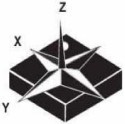
\includegraphics[width=6cm]{Images/HardwareDescription/MagnetometerDirection}
	\caption{\textbf{Magnetometer Directions}}
	\label{fig:Magnetometer}
	\cite{Stm:2015}
\end{figure}
\subsection{Description}
In the context of a magnetometer, the x, y, and z axes (Mx, My, Mz) typically delineate the three-dimensional space in which the magnetic field is being assessed. The x-axis typically corresponds to the horizontal component of the magnetic field, the y-axis signifies the vertical component, and the z-axis reflects the magnetic field strength \cite{Kostiainen:2023}. This three-dimensional measurement provides a comprehensive understanding of the magnetic field in the surrounding space.
A magnetometer is a sensor that measures the strength and direction of a magnetic field. It is commonly used to detect the Earth's magnetic field for navigation purposes, detect magnetic anomalies, or determine heading in devices like smartphones, drones, and robotics. Magnetometers are fundamental in compasses, GPS systems, and geological exploration (Ripka, 2001).
\subsection{Specific Sensors}
There are various types of magnetometers available, differing in precision, range, and applications. Here are some popular ones:
\begin{itemize}
	\item HMC5883L: A widely used 3-axis digital magnetometer that provides low-cost magnetic field measurement \cite{Honeywell:2012}.
	\item LSM303DLHC: Combines an accelerometer and magnetometer, enabling tilt-compensated compass applications \cite{Adafruit:2021a}.
	\item AK8963: A 3-axis magnetometer typically used with IMUs like the MPU9250 for high accuracy \cite{AsahiKasei:2014}.
	\item MAG3110: A small, low-power 3-axis magnetometer for embedded systems \cite{NXP:2013}.
\end{itemize}
\subsection{Specification}

General magnetometer specifications include:
\begin{itemize}
	\item 3D digital magnetic sensor: Detects magnetic fields with a full scale of ±4/±8/±12/±16 gauss.
	\item Axes: Single-axis or 3-axis (most modern sensors are 3-axis).
	\item Sensitivity: Ability to detect weak magnetic fields (e.g., microteslas, nanoteslas).
	\item Range: Typically between ±8 to ±100 microteslas.
	\item Resolution: The smallest change in the magnetic field that the sensor can detect.
	\item Power Consumption: Important for portable systems.
\item Interface: I2C, SPI, or analog output.
\end{itemize}
\subsection{Library}
Libraries simplify interfacing with magnetometer sensors, converting raw data into readable formats. Below are some libraries:

Arduino:
\begin{itemize}
	\item HMC5883L: Adafruit\_HMC5883\_Unified.h (Adafruit, 2021b).
	\item LSM303: Adafruit\_LSM303DLHC.h (Adafruit, 2021a).
\end{itemize}
Python:
\begin{itemize}
	\item Use smbus or CircuitPython libraries for I2C sensors \cite{Adafruit:2020}.
	\item Example for Raspberry Pi: hmc5883l Python library \cite{Hollingworth:2019}.
\end{itemize}
To install the library for Arduino:

\begin{verbatim}
// Include the necessary libraries
#include <Adafruit_Sensor.h>
#include <Adafruit_HMC5883_U.h>
\end{verbatim}

\subsection{Calibration}
Basic calibration steps:
\begin{itemize}
	\item Rotate the sensor in all directions.
	\item Plot the data to ensure it forms a circle.
	\item Apply corrections for centering the data.
\end{itemize}
\subsection{Simple Code}
\begin{code}[h!]
	\begin{Arduino}
	// Include the necessary libraries
	#include <Wire.h>
	#include <Adafruit_Sensor.h>
	#include <Adafruit_HMC5883_U.h>
	// Create an HMC5883 magnetometer object with a unique ID
	Adafruit_HMC5883_Unified mag = Adafruit_HMC5883_Unified(12345);
	// Setup function
	void setup(void) {
		// Start serial communication at 9600 baud rate
		Serial.begin(9600);
		// Initialize the magnetometer
		if (!mag.begin()) {
			Serial.println("No HMC5883L detected ... Check your wiring!");
			while (1);  // Halt the program if the sensor is not detected
		}
		
		// Set the magnetometer gain
		mag.setMagGain(HMC5883_MAGGAIN_1_3);
	}
	// Loop function
	void loop(void) {
		// Declare a variable to store magnetometer data
		sensors_event_t event;
		// Get the magnetometer event data
		mag.getEvent(&event);
		// Calculate the heading angle in radians
		float heading = atan2(event.magnetic.y, event.magnetic.x);
		if (heading < 0) heading += 2 * PI;
		// Convert the heading from radians to degrees
		float headingDegrees = heading * 180 / M_PI;
		// Print the heading in degrees
		Serial.println(headingDegrees);
		// Delay for 500ms before the next reading
		delay(500);
	}
	
	\end{Arduino}
	\caption{Example code for reading magnetometer data}\label{code:magnetometer-example}
\end{code}
\subsection{Applications}
Magnetometers have diverse applications, including:
\begin{itemize}
	\item Navigation: Electronic compasses in GPS, drones, and aircraft \cite{Sherwood:2013}.
	\item Robotics: Precise heading information for autonomous systems \cite{IEEE:2020}.
	\item Consumer Devices: Smartphones, wearables for direction detection \cite{AsahiKasei:2014}.
	\item Geological Exploration: Detect magnetic anomalies for mineral exploration \cite{Hansen:2017}.
	\item Space Exploration: Magnetic field mapping on planets.
	\item Security: Detection of ferromagnetic objects in metal detectors \cite{Williams:2015}.
\end{itemize}
\subsection{Tests}

The following C++ code reads and prints the magnetometer data (X, Y, Z values) from the LSM9DS1 sensor connected to the Arduino Nano 33 BLE Sense.

\begin{lstlisting}[caption={C++ Code for Arduino to Read Magnetometer Data}, label={lst:cpp_magnetometer}, style=pythonstyle]
	#include <Wire.h>
	#include <Adafruit_Sensor.h>
	#include <Adafruit_LSM9DS1.h>
	
	// Create an instance of the LSM9DS1 sensor
	Adafruit_LSM9DS1 lsm = Adafruit_LSM9DS1();
	
	void setup() {
		// Start serial communication
		Serial.begin(115200);
		
		// Initialize the LSM9DS1 sensor
		if (!lsm.begin()) {
			Serial.println("Could not find a valid LSM9DS1 sensor, check wiring!");
			while (1);
		}
		
		Serial.println("LSM9DS1 test initialized.");
	}
	
	void loop() {
		// Read magnetometer data
		sensors_event_t event;
		lsm.getEvent(&event, Adafruit_LSM9DS1::MAGNETOMETER);
		
		// Print magnetometer values
		Serial.print("Mag X: ");
		Serial.print(event.magnetic.x);
		Serial.print(" Y: ");
		Serial.print(event.magnetic.y);
		Serial.print(" Z: ");
		Serial.println(event.magnetic.z);
		
		// Delay before the next reading
		delay(1000);
	}
\end{lstlisting}

\newpage

This Python code reads the magnetometer data from the Arduino via serial communication.

\begin{lstlisting}[style=pythonstyle, caption={Python Code to Read Magnetometer Data via Serial}, label={lst:python_magnetometer}]
	import serial
	import time
	
	# Replace with the correct port for your system (e.g., 'COM3' on Windows or '/dev/ttyACM0' on Linux)
	arduino_port = '/dev/ttyACM0'  
	baud_rate = 115200
	
	# Establish connection to the Arduino
	arduino = serial.Serial(arduino_port, baud_rate, timeout=1)
	time.sleep(2)  # Wait for Arduino to initialize
	
	# Function to read magnetometer data from the Arduino
	def read_magnetometer():
	while True:
	line = arduino.readline().decode('utf-8').strip()
	if line:
	print(line)
	
	# Start reading magnetometer data
	read_magnetometer()
\end{lstlisting}

\subsection{Further Readings}
For more information, refer to:

Datasheets: Sensor-specific datasheets (e.g., HMC5883L, LSM303).
Books:
\begin{itemize}
	\item Ripka, A. (2001) Introduction to Magnetometers. New York: Wiley.
	\item Sherwood, T. (2013) Magnetic Sensors in Navigation Systems. Berlin: Springer.
\end{itemize}
Online Resources:
\begin{itemize}
	\item Adafruit tutorials on magnetometers \cite{Adafruit:2021a}.
	\item Research papers on magnetic anomaly detection \cite{Hansen:2017}.
\end{itemize}








